\chapter{Statistiek}

% \section{Introduction}

Wanneer ons 'n eksperiment uitvoer of 'n opname maak, kan ons potensieel met duisende of selfs miljoene waardes in die resulterende datastel sit. Te veel data kan oorweldigend wees en ons moet dit verminder of voorstel op 'n manier wat makliker is om te verstaan en te kommunikeer.\par 

Statistiek gaan oor die opsom van data. Statistiese metodes stel ons in staat om die noodsaaklike inligting in 'n datastel voor te stel en die onbelangrike inligting ter syde te stel. Ons moet versigtig wees om seker te maak dat ons statistiese metodes korrek toepas sodat onse nie per ongeluk sekere belangrike aspekte van die datastel uitlig en die data dus makliker maak om te interpreteer nie. \par

Deur statistiek oneerlik of swak toe te pas, kan ons belangrike inligting buite rekening laat en toelaat dat mense foutiewe gevolgtrekkings maak. \par

In hierdie hoofstuk gaan ons na 'n paar numeriese en grafiese metodes kyk waardeur data voorgestel kan word om dit makliker te maak om te interpreteer.\par


%The figure below shows one example of how we can reduce the complexity
%of a data set while still retaining the important information.

%FIGURE: Side-by-side images of two data sets drawn from the same $2$-d
%normal distribution. $N = 50$. Even though the individual data are
%different, the statistics (central tendency and dispersion) are very
%similar. The statistics capture the interesting aspects of the data.
%\begin{center}
%  \begin{tikzpicture}
%  \end{tikzpicture}
%\end{center}
\par
\chapterstartvideo{VMbqd}

\section{Versamelling van data}
\Definition{Data}{Data verwys na stukke inligting wat waargeneem en opgeteken kan word in 'n eksperiment of opname.}

Ons onderskei tussen twee soorte data: kwantitatiewe en kwalititiewe data. Data is die meervoud van 'datum' en dus is dit 'n meervoudsvorm: in Engels s\^e ons 'the data are' en nie 'the data is' nie.

\Definition{Kwantitatiewe data}{Kwantitatiewe data kan as getalle geskryf word.}

Kwantitatiewe data kan diskreet of kontinu wees. Diskrete kwantitatiewe data kan voorgestel word deur heelgetalle en kom gewoonlik voor wanneer ons dinge tel, byvoorbeeld die aantal SMS-boodskappe gestuur op een dag.\par

Kontinue kwantitatiewe data kan voorgestel word deur re\"ele getalle, byvoorbeeld die hoogte of die massa van 'n persoon, die afstand afgel\^e deur 'n motor of die tydsduur van 'n telefoonoproep.

\Definition{Kwalitatiewe data}{Kwalitatiewe data is data wat nie as getalle geskryf kan word nie, byvoorbeeld die insameling van die antwoorde van mense oor hoe hulle voel of wat hulle geliefkoosde kleur is.}

Kategoriale data en anekdotiese data is twee algemene tipes kwalitatiewe data. Kategoriale data kan kom van ’n beperkte aantal moontlikhede, byvoorbeeld jou geliefkoosde koeldrank, die kleur van jou selfoon of jou moedertaal. \par

Anekdotiese data neem die vorm aan van ’n onderhoud of ’n storie, byvoorbeeld wanneer jy iemand vra wat hulle persoonlike ondervinding was toe hulle ’n sekere produk gebruik het, of wat hulle dink van iemand anders se optrede. \par

Kategoriale data kan soms omgeskakel word na kwantitatiewe data deur die aantal kere te tel wat elke kategorie voorkom. In ’n klas met $30$ leerders, vra ons elkeen wat die kleur is van sy of haar selfoon en ons kry die volgende antwoorde:

  \begin{center}
    \begin{tabular}{|c|c|c|c|c|c|c|c|c|c|}\hline
     
      swart & swart & swart & wit & pers & red & red & swart & swart & swart \\ \hline
      wit & wit & swart & swart & swart & swart & pers & swart & swart & wit \\ \hline
      pers & swart & rooi & rooi & wit & swart & oranje & oranje & swart & wit \\ \hline
     
    \end{tabular}
  \end{center}

Hierdie is ‘n kategoriale kwantitatiewe datastel aangesien elkeen van die antwoorde kom uit een van ’n klein aantal moontlikhede. Ons kan dieselfde data voorstel deur te tel hoeveel kere elke kleur voorkom.

  \begin{center}
    \begin{tabular}{|c|c|}\hline
      
      \textbf{Kleur} & \textbf{Telling} \\ \hline

      swart & 15 \\ \hline
      wit & 6 \\\hline
      rooi & 4 \\\hline
      pers & 3 \\\hline
      oranje & 2\\
    \hline
    \end{tabular}
  \end{center}

  Dit is diskrete kwantitatiewe data aangesien elke telling 'n heelgetal is.

\begin{wex}{Kwantitatiewe data}
{Thembisile stel belang daarin om lugtyd te her-verkoop aan haar klasmaats. Sy wil graag weet hoeveel besigheid sy van hulle kan verwag. Daarom vra sy elk van sy $20$ klasmaats hoeveel SMS-boodskappe hulle gestuur het gedurende die vorige dag. Die resultate was:
\\

    \begin{center}
      \begin{tabular}{|c|c|c|c|c|c|c|c|c|c|}\hline
        $20$ & $ 3$ & $ 0$ & $14$ & $30$ & $9$ & $11$ & $13$ & $13$ & $15$ \\ \hline
         $9$ & $13$ & $16$ & $12$ & $13$ & $7$ & $17$ & $14$ & $ 9$ & $13$ \\ \hline
        
      \end{tabular}
    \end{center}
    \vspace{8pt}\\

    Is hierdie datastel kwalitatief of kwantitatief? Verduidelik jou antwoord.
}{

  Die aantal SMS-boodskappe is 'n getal, wat beteken die data is kwantitatief en diskreet.
}
\end{wex}

\begin{wex}{Kwalitatiewe of kwantitatiewe data}
{Thembisile wil uitvind wat die mees gewilde selfoon verskaffer is onder leerders in haar skool. Hierdie keer kies Thembisile op willekeurige wyse $20$ leerders uit die hele skool en vra aan hulle watter selfoon verskaffer hulle tans gebruik.
 Die $20$ resultate was:

    \begin{center}
      \begin{tabular}{|p{0.17\textwidth}|p{0.17\textwidth}|p{0.17\textwidth}|p{0.17\textwidth}|p{0.17\textwidth}|}\hline
        
        Cell C & Vodacom & Vodacom & MTN & Vodacom \\\hline
        MTN & MTN & Virgin Mobile & Cell C & 8-ta \\\hline
        Vodacom & MTN & Vodacom & Vodacom & MTN \\\hline
        Vodacom & Vodacom & Vodacom & Virgin Mobile & MTN \\\hline
      \end{tabular}
    \end{center}
\vspace{8pt}\\
    Is hierdie datastel kwalitatief of kwantitatief? Verduidelik jou antwoord.
}{

  Aangesien die antwoorde nie getalle is nie maar een van 'n klein aantal moontlikhede word hierdie kategoriale kwalitatiewe data genoem.
}
\end{wex}

\section{Maatstawwe van sentrale neiging}

\subsection{Gemiddelde}
\Definition{Gemiddelde}{Die gemiddelde word gedefinieer as die som van 'n stel datawaardes, gedeel deur die aantal waardes in die som. 'n Horisontale strepie oor 'n veranderlike is die notasie wat gebruik word vir die gemiddelde van stel datawaardes. Die formule vir die gemiddelde van 'n datastel $\{x_1;
  x_2; \ldots; x_n\}$ is
  \begin{align*}
    \overline{x} &= \frac{1}{n}\sum_{i=1}^n x_i \\
                 &= \frac{x_1 + x_2 + \cdots + x_n}{n}
  \end{align*}
}

Die gemiddelde word soms die rekenkundige gemiddelde genoem.
\par
\mindsetvid{Mean, median and mode}{VMbqd}

\begin{wex}{Berekening van die gemiddelde}
{Wat is die gemiddelde van die datastel $\{10;\ 20;\ 30;\ 40;\ 50\}$?}
{
  \westep{Bereken die som van die data}
  \begin{equation*}
    10 + 20 + 30 + 40 + 50 = 150
  \end{equation*}

  \westep{Deel die som deur die getal datapunte in die stel om die gemiddelde te kry}

  Aangesien daar $5$ waardes in die datastel is, het ons
  \begin{equation*}
    \mbox{Gemiddelde} = \frac{150}{5} = 30
  \end{equation*}
}
\end{wex}

\subsection{Mediaan}
\Definition{Mediaan}
{Die mediaan van 'n datastel is die waarde van die sentrale of middelste datapunt wanneer die datastel georden word van die kleinste tot die grootste waarde.}

Presies die helfte van die datawaardes is kleiner as die mediaan en die ander helfte is groter as die mediaan.\par

Om die mediaan van 'n kwantitatiewe datastel te bereken, sorteer die data van die kleinste tot die grootste waarde en vind dan die waarde in die middel (middelwaarde). As daar 'n ewe aantal datapunte is, sal die mediaan halfpad tussen twee waardes in die datastel wees.

\begin{wex}{Mediaan van 'n onewe aantal datawaardes}
{Wat is die mediaan van $\{10;\ 14;\ 86;\ 2;\ 68;\ 99;\ 1\}$?}
{
  \westep{Orden die waardes}

  Die waardes in die datastel, van die kleinste tot die grootste is
  \begin{equation*}
    1;\ 2;\ 10;\ 14;\ 68;\ 86;\ 99
  \end{equation*}

  \westep{Vind die middelwaarde (getal in die middel)}

  Daar is $7$ waardes in die datastel. Aangesien daar 'n onewe aantal datawaardes is, sal die mediaan gelyk wees aan die waarde in die middelste, dus die $4^{de}$, posisie. Dus is $14$ die mediaan van die datastel.
}
\end{wex}

\begin{wex}{Mediaan vir 'n ewe aantal waardes}
{Wat is die mediaan van $\{11;\ 10;\ 14;\ 86;\ 2;\ 68;\ 99;\ 1\}$?}
{
  \westep{Orden die waardes}

  Die waardes in die datastel, van klein na groot, is
  \begin{equation*}
    1;\ 2;\ 10;\ 11;\ 14;\ 68;\ 86;\ 99
  \end{equation*}

  \westep{Vind die middelwaarde}
  Daar is $8$ waardes in die datastel. Omdat daar 'n ewe aantal \newline
datawaardes is, sal die mediaan halfpad tussen die twee waardes in die middel wees. Dit is naamlik die $4^{de}$ en $5^{de}$ posisies. Die waarde in die 
  $4^{de}$ posisie is $11$ en die waarde in die $5^{de}$ posisie is
  $14$. Die mediaan l\^e halfpad tussen die twee en is dus
  \begin{equation*}
    \mbox{Mediaan} = \frac{11+14}{2} = 12,5
  \end{equation*}
}
\end{wex}

\subsection{Modus}
\Definition{Modus}
{Die modus van 'n datastel is die waarde wat die meeste voorkom in die stel. Die modus kan ook beskryf word as die mees algemene waarde met die hoogste voorkomsfrekwenie in die datastel.}

Om die modus te bereken, tel ons doodeenvoudig die aantal kere wat elke datawaarde in die datastel voorkom en vind so die waarde wat die meeste kere voorkom.\par

‘n Datastel kan meer as een modus hê as daar meer as een waarde is wat die hoogste telling het. Byvoorbeeld, beide $2$ en $3$ is modi (modusse) in die datastel $\{1;\ 2;\ 2;\ 3;\ 3\}$. As alle punte in die datastel met dieselfde frekwensie voorkom, kan ons die datastel beskryf as een met baie modusse of een met geen modus nie. 

\begin{wex}{Vind die modus}
{Vind die modus van die datastel $\{2;\ 2;\ 3;\ 4;\ 4;\ 4;\ 6;\ 6;\ 7;\ 8;\ 8;\ 10;\ 10\}$.}
{
  \westep{Tel die aantal kere wat elke waarde voorkom in die datastel}
\\
  \begin{center}
    \begin{tabular}{|c|c|} \hline
      \textbf{Waarde} & \textbf{Telling} \\ \hline

      $2$ & $2$ \\ \hline
      $3$ & $1$ \\\hline 
      $4$ & $3$ \\\hline
      $6$ & $2$ \\\hline
      $7$ & $1$ \\\hline
      $8$ & $2$ \\\hline
      $10$ & $2$ \\\hline

    \end{tabular}
  \end{center}

  \westep{Vind die waarde wat die meeste kere voorkom}

  Van die af bostaande tabel kan ons sien $4$ is die enigste waarde wat $3$ keer voorkom en al die ander datawaardes kom minder kere voor. Dus is $4$ die modus van die datastel.
}
\end{wex}

Een probleem met die gebruik van die modus as ’n maatstaf van sentrale neiging, is dat ons gewoonlik nie die modus van ’n kontinue datastel kan bereken nie. Aangesien kontinue waardes op enige plek op die reële getallelyn kan lê, sal enige spesifieke waarde omtrent nooit herhaal word nie. Dit beteken dat die frekwensie van elke waarde in die datastel $1$ sal wees en dat daar dus geen modus sal wees nie. Een manier om hierdie probleem aan te spreek is met groepering van data.

\clearpage
\begin{wex}{
Vergelyk maatstawwe van sentrale neiging
% Comparison of measures of central tendency
}
{Om verbruikers te beskerm is daar in Suid-Afrika regulasies ten opsigte van die vervaardiging van brood. Volgens wet moet ’n brood, waarop die massa nie spesifiek aangedui is nie, $800$ g weeg met ’n speling van $5$ persent onder en $10$ persent bokant hierdie massa. Vishnu is geïnteresseerd daarin om uit te vind hoe ’n nasionale verskaffer voldoen aan die standaarde. Hy het die plaaslike tak van die verskaffer besoek en die massas van $10$ verskillende brode vir ’n week lank aangeteken. Hier is die resultate, in gram:\\
\vspace*{-20pt}
    \begin{center}
      \begin{tabular}{|c|c|c|c|c|c|c|} \hline
       
        \textbf{Maandag} & \textbf{Dinsdag} & \textbf{Woensdag} & \textbf{ Donderdag} & \textbf{Vrydag} & \textbf{Saterdag} & \textbf{Sondag} \\ \hline
        
        $802,4$ & $787,8$ & $815,7$ & $807,4$ & $801,5$ & $786,6$ & $799,0$ \\ \hline
        $796,8$ & $798,9$ & $809,7$ & $798,7$ & $818,3$ & $789,1$ & $806,0$ \\ \hline
        $802,5$ & $793,6$ & $785,4$ & $809,3$ & $787,7$ & $801,5$ & $799,4$ \\ \hline
        $819,6$ & $812,6$ & $809,1$ & $791,1$ & $805,3$ & $817,8$ & $801,0$ \\ \hline
        $801,2$ & $795,9$ & $795,2$ & $820,4$ & $806,6$ & $819,5$ & $796,7$ \\ \hline
        $789,0$ & $796,3$ & $787,9$ & $799,8$ & $789,5$ & $802,1$ & $802,2$ \\ \hline
        $789,0$ & $797,7$ & $776,7$ & $790,7$ & $803,2$ & $801,2$ & $807,3$ \\ \hline
        $808,8$ & $780,4$ & $812,6$ & $801,8$ & $784,7$ & $792,2$ & $809,8$ \\ \hline
        $802,4$ & $790,8$ & $792,4$ & $789,2$ & $815,6$ & $799,4$ & $791,2$ \\ \hline
        $796,2$ & $817,6$ & $799,1$ & $826,0$ & $807,9$ & $806,7$ & $780,2$ \\ \hline
       
      \end{tabular}
    \end{center}
% \vspace{8pt}\\
\begin{minipage}{0.9\textwidth}
    \begin{enumerate}[noitemsep, label=\textbf{\arabic*}.]
    \item Is hierdie datastel kwalitatief of kwantitatief? Verduidelik jou antwoord.
    \item Bepaal die gemiddelde, mediaan en modus van die massa van ’n brood vir elke dag van die week. Gee jou antwoorde tot een desimale plek.
    \item Gebaseer op hierdie data, dink jy die verskaffer voorsien brood wat voldoen aan die Suid-Afrikaanse riglyne?
    \end{enumerate}
\end{minipage}
}{
  \westep{Kwalitatief of kwantitatief?}

  Aangesien enige massa verteenwoordig word deur ’n getal, is die datastel kwantitatief. Omdat die massa enige reële getal kan wees, is die data kontinu.

  \westep{Bereken die gemiddelde}

 In elke kolom, vir elke dag van die week, tel ons die datawaardes bymekaar en verdeel die totaal deur die aantal datapunte, naamlik $10$.

  Vir Maandag is die som van massas $8~007,9$ g, dus is die gemiddelde vir Maandag:
  \begin{equation*}
    \frac{8~007,9}{10} = 800,8\mbox{ g}
  \end{equation*}

  Op dieselfde manier kan ons die gemiddelde vir elke dag van die week bereken. Sien die tabel hieronder vir die resultate.

  \westep{Bereken die mediaan}

  In elke kolom sorteer ons die waardes van die laagste tot die hoogste en vind die waarde in die middel. Aangesien daar ’n ewe aantal metings, naamlik 10, is die mediaan halfpad tussen die twee getalle in die middel.

  Vir Maandag is die gesorteerde lys van getalle:

  \begin{equation*}
    789,0;\ 789,0;\ 796,2;\ 796,7;\ 801,2;\ 802,3;\ 802,3;\ 802,5;\ 808,7;\ 819,6
  \end{equation*}

  Die twee waardes in die middel is $801,2$ en $802,3$ dus is die mediaan
  \begin{equation*}
    \frac{801,2 + 802,3}{2} = 801,8\mbox{ g}
  \end{equation*}

  Op dieselfde wyse kan ons die mediaan bereken vir elke dag van die week. Hier is die tabel met al die gemiddeldes en mediane. 
\\
  \begin{center}
    \begin{tabular}{|c|c|c|} \hline
      \textbf{Dag} & \textbf{Gemiddelde} &\textbf{Mediaan} \\  \hline
      Maandag & $800,8$ g & $801,8$ g \\ \hline
      Dinsdag & $797,2$ g & $796,1$ g \\ \hline
      Woensdag & $798,4$ g & $797,2$ g \\ \hline
      Donderdag & $803,4$ g & $800,8$ g \\ \hline
      Vrydag & $802,0$ g & $804,3$ g \\ \hline
      Saterdag & $801,6$ g & $801,4$ g \\ \hline
      Sondag & $799,3$ g & $800,2$ g \\ \hline
    \end{tabular}
  \end{center}
\vspace{8pt}\\
  Uit bostaande berekeninge kan ons sien dat die gemiddelde en die mediaan naby aan mekaar, maar nie heeltemal dieselfde  is nie. In die volgende voorbeeld sal ons sien dat die gemiddelde en die mediaan nie altyd naby aan mekaar is nie.

  \westep{Bepaal die modus}

  Aangesien die data kontinu is, kan ons nie die modus bereken nie. In die volgende afdeling sal ons sien hoe om data te groepeer om dit moontlik te maak om ’n benadering vir die modus te bereken.

  \westep{Gevolgtrekking: is die vervaardiger betroubaar?}

  In hierdie geval is die vereiste dat die massa van ’n brood tussen $800$ g minus $5$\%, dus $760$ g, en $800$ g plus 
  $10$\%, dus $880$ g sal wees. Aangesien al Vishnu se metings binne hierdie grense val en aangesien die gemiddeldes en die mediane almal naby aan $800$ g is, kan ons tot die gevolgtrekking kom dat die verskaffer betroubaar is.
}
\end{wex}

\Definition{Uitskieter}{’n Uitskieter is ’n waarde in die datastel wat nie tipies is van die res van die stel nie. Dit is gewoonlik ’n waarde wat baie groter is of baie kleiner is as al die ander waardes in die stel.}
\clearpage
\begin{wex}{Invloed van die uitskieters op die gemiddelde en die mediaan}
{Die lengtes van $10$ leerders word in sentimeters gemeet en gee die volgende datastel:
    \begin{equation*}
      \{150;\ 172;\ 153;\ 156;\ 146;\ 157;\ 157;\ 143;\ 168;\ 157\}
    \end{equation*}
    Later voeg ons nog ’n leerder, met die uitsonderlike lengte van $181$ cm, by hierdie groep.

   Vergelyk die gemiddelde en mediaan van die lengtes van die leerders voor en na die laaste leerder bygevoeg is.
}{
  \westep{Bereken die gemiddelde van die eerste $10$ leerders}

  \begin{align*}
    
\mbox{Gemid. } &= \frac{150 + 172 + 153 + 156 + 146 + 157 + 157 + 143 + 168 + 157}{10}\\
    &= 155,9\mbox{ cm}
  \end{align*}

  \westep{Bereken die gemiddelde van al $11$ leerders}

  \begin{align*}
   
\mbox{Gemid. } &= \frac{150 + 172 + 153 + 156 + 146 + 157 + 157 + 143 + 168 + 157 + 181}{11}\\
    &= 158,2\mbox{ cm}
  \end{align*}

  Hieruit sien ons die gemiddelde lengte verander met 
  $158,2 - 155,9 = 2,3\mbox{ cm}$ wanneer ons die uitskieter (die lang leerder) byvoeg by die datastel.

  \westep{Bereken die mediaan van die eerste $10$ leerders}

  Om die mediaan te vind, moet ons die datastel sorteer:
  \begin{equation*}
    \{143;\ 146;\ 150;\ 153;\ 156;\ 157;\ 157;\ 157;\ 168;\ 172\}
  \end{equation*}
  Aangesien daar ’n ewe getal waardes is, naamlik 10, lê die mediaan halfpad tussen die $5^{de}$ en $6^{de}$ waardes:
  \begin{equation*}
    \mbox{Mediaan} =\frac{156+157}{2} = 156,5\mbox{ cm}
  \end{equation*}

  \westep{Bereken die mediaan van al $11$ leerders}

  Nadat die lang leerder bygevoeg is, sien die gesorteerde datastel as volg daaruit:
  \begin{equation*}
    \{143;\ 146;\ 150;\ 153;\ 156;\ 157;\ 157;\ 157;\ 168;\ 172;\ 181\}
  \end{equation*}
  Met $11$ waardes in die datastel is die mediaan die $6^{de}$ waarde: $157$ cm.
  Dus verander die mediaan net met $0,5$ cm wanneer ons die uitskieter by die datastel voeg.

 In die algemeen, word die mediaan minder beïnvloed deur die byvoeging van uitskieters by ’n datastel, as die gemiddelde. Dit is belangrik omdat dit redelik algemeen is dat uitskieters gemeet word tydens ’n eksperiment as gevolg van probleme met toerusting of onverwagte versteurings.
}
\end{wex}

\begin{exercises}{}{
    \begin{enumerate}[noitemsep, label=\textbf{\arabic*}.]

    \item Bereken die gemiddelde, die mediaan en die modus van die volgende datastelle:
      \begin{enumerate}[noitemsep, label=\textbf{(\alph*)} ]
      \item $2;~5;~8;~8;~11;~13;~22;~23;~27$
      \item $15;~17;~24;~24;~26;~28;~31;~43$
      \item $4;~11;~3;~15;~11;~13;~25;~17;~2;~11$
      \item $24;~35;~28;~41;~32;~49;~31$
      \end{enumerate}
    \item Die ouderdomme van $15$ drawwers van die  Comrades Marathon is aangeteken:
      \begin{equation*}
        31;~42;~28;~38;~45;~51;~33;~29;~42;~26;~34;~56;~33;~46;~41
      \end{equation*}
      Bereken die gemiddelde, die mediaan en die modus van die ouderdomme.
    \item In die eerste van ’n aantal flesse is daar $1$ lekker. In die tweede is daar $3$ lekkers. Die gemiddelde van die aantal lekkers in die eerste twee flesse is $2$.
      \begin{enumerate}[noitemsep, label=\textbf{(\alph*)} ]
      \item As die gemiddelde aantal lekkers in die eerste drie flesse $3$ is, hoeveel lekkers is daar in die derde fles?
      \item As die gemiddelde aantal lekkers in die eerste vier flesse $4$ is, hoeveel lekkers is daar in die vierde fles?
      \end{enumerate}
    \item Vind ’n stel van 5 ouderdomme waarvoor die gemiddelde ouderdom $5$ is, die modale ouderdom (dus die modus) $2$ is en die mediaan ouderdom $3$ jaar is.
    \item Vier vriende het elkeen ’n aantal albasters. Hulle bereken dat $10$ die gemiddelde is van die aantal albasters wat hulle het. Een van hulle vertrek. Sy het $4$ albasters. Hoeveel albasters het die oorblywende vriende altesaam?
    \end{enumerate}
% Automatically inserted shortcodes - number to insert 5
\par \practiceinfo
\par \begin{tabular}[h]{cccccc}
% Question 1
(1.)	02qr	&
% Question 2
(2.)	02qs	&
% Question 3
(3.)	02qt	&
% Question 4
(4.)	02qu	&
% Question 5
(5.)	02qv	&
\end{tabular}
% Automatically inserted shortcodes - number inserted 5
% \practiceinfo
% \par 
% \par \begin{tabular}[h]{cccccc}
% (1.) 00jr&  (2.) 00js&  (3.) 00jt&  (4.) 00ju&  (5.) 00jv\end{tabular}
}
\end{exercises}

\section{Groepering van data}
\label{sec:statistics_grouping_data}
'n Algemene manier om kwantitatiewe data te hanteer is om die volle stel waardes te onderverdeel in ’n aantal sub-groepe of klasse. Deur elke kontinue datawaarde in te deel in die klas waarin dit val, verander die data in die stel van kontinu na diskreet.\par
%We will see below that this has some benefits, but we gain the
%benefits at the cost of losing some information.

Groepering word gedoen deur ’n stel klasse te definieer en dan te tel hoeveel data in elke klas val. Die klasse moet so gekies word dat hulle nie oorvleuel nie en sodat hulle die volle wydte van die datastel dek.\par

Een manier om gegroepeerde data voor stel is met ’n histogram. ’n Histogram is ’n versameling van reghoeke, waar die basis van elke reghoek (op die $x$-as) die waardes dek in die klas wat daaraan gekoppel is en die hoogte van die reghoek ooreenstem met die aantal waardes in die klas. 
\par
\mindsetvid{Grouping data}{VMbue}

\begin{wex}{Groepe en histogramme}
{Die hoogtes van $30$ leerders word in sentimeters gegee, in die tabel hieronder.
\\
    \begin{center}
      \begin{tabular}{|c|c|c|c|c|c|c|c|c|c|}\hline
   
        $142$ & $163$ & $169$ & $132$ & $139$ & $140$ & $152$ & $168$ & $139$ & $150$\\ \hline
        $161$ & $132$ & $162$ & $172$ & $146$ & $152$ & $150$ & $132$ & $157$ & $133$\\ \hline
        $141$ & $170$ & $156$ & $155$ & $169$ & $138$ & $142$ & $160$ & $164$ & $168$\\ \hline
 
      \end{tabular}
    \end{center}
\vspace {8pt}\\
    Groepeer die data in die volgende klasse en trek ’n histogram van die gegroepeerde data:
    \begin{align*}
      130 &\leq h < 140 \\
      140 &\leq h < 150 \\
      150 &\leq h < 160 \\
      160 &\leq h < 170 \\
      170 &\leq h < 180
    \end{align*}
    (Let daarop dat die data nie oorvleuel waar een klas eindig en die volgende klas begin nie.)
}{
  \westep{Tel die aantal datawaardes in elke klas}
  \begin{center}
    \begin{tabular}{|c|c|} \hline

      \textbf{Gebied} & \textbf{Telling} \\ \hline
    
      $130 \leq h < 140$ & $7$ \\ \hline
      $140 \leq h < 150$ & $5$ \\\hline
      $150 \leq h < 160$ & $7$ \\\hline
      $160 \leq h < 170$ & $9$ \\\hline
      $170 \leq h < 180$ & $2$ \\\hline

    \end{tabular}
  \end{center}
  
  \westep{Trek die histogram}

  Aangesien daar $5$ klasse is, sal ons histogram uit $5$ reghoeke bestaan. Die basis van elke reghoek word deur die klaswydte gedefinieer. Die hoogte van elke reghoek word gedefineer deur die datatelling in die klas.
  
  \begin{center}
    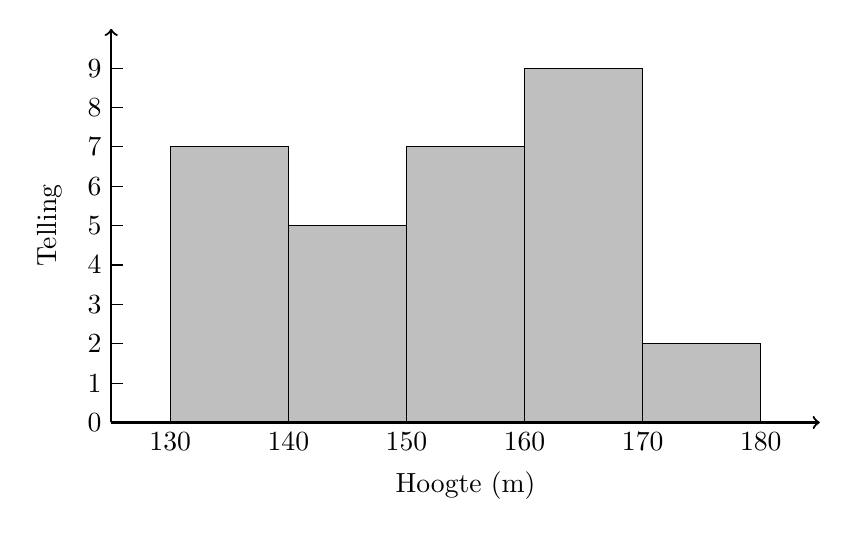
\begin{tikzpicture}[xscale=0.15,yscale=0.5]
      \draw[fill=lightgray] (130,0) rectangle (140,7);
      \draw[fill=lightgray] (140,0) rectangle (150,5);
      \draw[fill=lightgray] (150,0) rectangle (160,7);
      \draw[fill=lightgray] (160,0) rectangle (170,9);
      \draw[fill=lightgray] (170,0) rectangle (180,2);

\draw[thick,->] (125,0) -- (185,0) node[anchor=north] {};
      % x labels
      \foreach \x in {130, 140, ..., 180} {
        \draw (\x,0) node[anchor=north] {$\x$};
      }

      % y axis
      \draw[thick,->] (125,0) -- (125,10) node[midway,sloped,anchor=south,yshift=0.5cm] {Telling};
      % y labels
      \foreach \y in {0, 1, ..., 9} {
        \draw (125,\y) node[anchor=east] {$\y$} -- (126,\y);
      }
      % axis labels
      \draw (155, -1) node[anchor=north] {Hoogte (m)};
    \end{tikzpicture}
  \end{center}

  Die histogram maak dit maklik om te sien in watter klas die meeste lengtes val en gee ’n oorsig oor die verspreiding van die waardes in die datastel.
}
\end{wex}    

\begin{exercises}{}{
    \begin{enumerate}[itemsep=5pt, label=\textbf{\arabic*}. ]
    \item ’n Eksperiment is onderneem in die skool en $50$ leerders is gevra om te raai hoeveel lekkers daar in ’n bottel is. Die volgende raaiskote word aangeteken:
      \\
      \begin{center}
        \begin{tabular}{|c|c|c|c|c|c|c|c|c|c|} \hline
          $56$ & $49$ & $40$ & $11$ & $33$ & $33$ & $37$ & $29$ & $30$ & $59$ \\ \hline
          $21$ & $16$ & $38$ & $44$ & $38$ & $52$ & $22$ & $24$ & $30$ & $34$ \\\hline
          $42$ & $15$ & $48$ & $33$ & $51$ & $44$ & $33$ & $17$ & $19$ & $44$ \\\hline
          $47$ & $23$ & $27$ & $47$ & $13$ & $25$ & $53$ & $57$ & $28$ & $23$ \\\hline
          $36$ & $35$ & $40$ & $23$ & $45$ & $39$ & $32$ & $58$ & $22$ & $40$ \\\hline
        \end{tabular}
      \end{center}
      \vspace{8pt}\\

      \begin{enumerate}[noitemsep, label=\textbf{(\alph*)} ]
      \item Trek ’n gegroepeerde frekwensietabel op en gebruik die volgende intervalle
        $10 < x \leq 20$;\ $20 < x \leq 30$;\ $30 < x \leq 40$;\ 
        $40 < x \leq 50$; en \ $50 < x \leq 60$.
      \item Trek ’n histogram om die frekwensietabel van die gegroepeerde data voor te stel.
      \end{enumerate}
    \end{enumerate}
% Automatically inserted shortcodes - number to insert 1
\par \practiceinfo
\par \begin{tabular}[h]{cccccc}
% Question 1
(1.)	02qw	&
\end{tabular}
% Automatically inserted shortcodes - number inserted 1
% \practiceinfo
% \par 
% \par \begin{tabular}[h]{cccccc}
% (1.) 00jw& \end{tabular}
}
\end{exercises}
% 
 %Put this in other text flows straight out of previous exercises?!?!
\subsection*{Maatstawwe van sentrale neiging}
Ons beramings van maatstawwe van sentrale neiging sal verander as ons data groepeer omdat ons sekere inligting verloor wanneer ons data in klasse indeel. As ons slegs die gegroepeerde data het om mee te werk, het ons nie meer die gemete waardes van die data tot dieselfde vlak van akkuraatheid as vantevore nie. Die beste wat ons kan doen is om te aanvaar dat die waardes gegroepeer is in die middel van elke klas.\par

As ons terugkyk na die vorige voorbeeld , sien ons ons het met ’n datastel van leerders se hoogtes begin
\begin{align*}
  \{&132;\ 132;\ 132;\ 133;\ 138;\ 139;\ 139;\ 140;\ 141;\ 142;\ 142;\ 146;\ 150;\ 150;\ 152;\\
    &152;\ 155;\ 156;\ 157;\ 160;\ 161;\ 162;\ 163;\ 164;\ 168;\ 168;\ 169;\ 169;\ 170;\ 172\}
\end{align*}
Let daarop dat die data hier gesorteer is.

Die gemiddelde van hierdie data is $151,8$ en die mediaan is $152$. Die modus is $132$, maar onthou dat daar probleme is met die berekening van die modus van kontinue kwantitatiewe data. \par

Na groepering van die data, het ons nou die datastel hieronder aangetoon. Let daarop dat elke datawaarde geplaas word in die middel van die klas en dat die aantal kere wat elke datawaarde herhaal word presies ooreenstem met die telling in elke klas. 
\begin{align*}
  \{&135;\ 135;\ 135;\ 135;\ 135;\ 135;\ 135;\ 145;\ 145;\ 145;\ 145;\ 145;\ 155;\ 155;\ 155;\\
    &155;\ 155;\ 155;\ 155;\ 165;\ 165;\ 165;\ 165;\ 165;\ 165;\ 165;\ 165;\ 165;\ 175;\ 175\}
\end{align*}
Die groepering verander die maatstawwe van sentrale neiging aangesien elke datawaarde nou hanteer word asof dit geleë is in die middel van die klas waarin dit geplaas is. \par
\clearpage
Die gemiddelde is nou $153$, die mediaan is $155$ en die modus is $165$. Dit is eintlik ’n beter benadering van die modus aangesien die groepering getoon het in watter klas die meeste leerderlengtes val. 


\begin{exercises}{}{
  \begin{enumerate}[itemsep=8pt, label=\textbf{\arabic*}.]

  \item Oorweeg die volgende gegroepeerde data en bereken die gemiddelde, die modale groep en die mediaangroep.
\\
    \begin{center}
      \begin{tabular}{|c|c|}\hline
      
        \textbf{Massa (kg)} & \textbf{Telling} \\\hline
     
        $40 < m \leq 45$ & $7$ \\\hline
        $45 < m \leq 50$ & $10$ \\\hline
        $50 < m \leq 55$ & $15$ \\\hline
        $55 < m \leq 60$ & $12$ \\\hline
        $60 < m \leq 65$ & $6$ \\\hline
  
      \end{tabular}
    \end{center}

  \item Vind die gemiddelde, die modale groep en die mediaangroep in die datastel van die tyd wat mense benodig om ’n spel te voltooi:
\\
    \begin{center}
      \begin{tabular}{|c|c|} \hline

       \textbf{Tyd (s)} & \textbf{Telling} \\ \hline

        $35 < t \leq 45$ & $5$ \\\hline
        $45 < t \leq 55$ & $11$ \\\hline
        $55 < t \leq 65$ & $15$ \\\hline
        $65 < t \leq 75$ & $26$ \\\hline
        $75 < t \leq 85$ & $19$ \\\hline
        $85 < t \leq 95$ & $13$ \\\hline
        $95 < t \leq 105$ & $6$ \\\hline

      \end{tabular}
    \end{center}
% Still in English
\item Die histogram hieronder bewys die aantal passasiers wat per week in Alfred se taxi reis.\\
Bereken:
\begin{enumerate}[noitemsep, label=\textbf{(\alph*)} ]
\item die modale interval
\item die totale aantal passasiers wat in Alfred se taxi gereis het
\item 'n beraming van die gemiddelde
\item 'n beraming van die mediaan
\item indien dit geskat word dat elke passasier 'n gemiddelde afstand van $5$ km gereis het, hoeveel geld sou Alfred verdien as hy R~$3,50$ per km gevra het?
\end{enumerate}
\begin{center}
\scalebox{1} % Change this value to rescale the drawing.
{
\begin{pspicture}(0,-5.1475)(9.378126,5.1075)
\definecolor{color5165b}{rgb}{0.7725490196078432,0.7725490196078432,0.7725490196078432}
\rput(1.3781264,-3.8925){\psaxes[linewidth=0.028222222,arrowsize=0.05291667cm 2.0,arrowlength=1.4,arrowinset=0.4,tickstyle=bottom,ticksize=0.10583333cm,dx=1.0cm,dy=1.0cm,Dx=100,Dy=2,Ox=300]{<->}(0,0)(-1,-1)(8,9)}
\psframe[linewidth=0.02,dimen=outer,fillstyle=solid,fillcolor=color5165b](3.392293,-1.8890625)(2.372293,-3.8890624)
\psframe[linewidth=0.02,dimen=outer,fillstyle=solid,fillcolor=color5165b](4.412293,-0.8890625)(3.372293,-3.8890624)
\psframe[linewidth=0.02,dimen=outer,fillstyle=solid,fillcolor=color5165b](5.412293,2.1309376)(4.372293,-3.8890624)
\psframe[linewidth=0.02,dimen=outer,fillstyle=solid,fillcolor=color5165b](6.392293,4.1309376)(5.372293,-3.8890624)
\psframe[linewidth=0.02,dimen=outer,fillstyle=solid,fillcolor=color5165b](7.392293,0.1309375)(6.372293,-3.8890624)
\psframe[linewidth=0.02,dimen=outer,fillstyle=solid,fillcolor=color5165b](8.392293,-2.8690624)(7.372293,-3.8890624)
% \usefont{T1}{ptm}{m}{n}
\rput(5.369637,-4.9225){Aantal passasiers}
% \usefont{T1}{ptm}{m}{n}
\rput{89.854546}(0.73185694,0.38878262){\rput(0.13573053,0.5775){Telling}}
\end{pspicture} 
}
\end{center}
  \end{enumerate}
% Automatically inserted shortcodes - number to insert 3
\par \practiceinfo
\par \begin{tabular}[h]{cccccc}
% Question 1
(1.)	02qx	&
% Question 2
(2.)	02qy	&
% Question 3
(3.)	02qz	&
\end{tabular}
% Automatically inserted shortcodes - number inserted 3
% \practiceinfo
% \par 
% \par \begin{tabular}[h]{cccccc}
% (1.) 00jx&  (2.) 00jy&  (3.) 00jz\end{tabular}

}
\end{exercises}

\section{Spreiding}
Die sentrale neiging is nie die enigste interessante of nutting inligting van ’n datastel nie. Die twee datastelle hieronder het dieselfde gemiddelde, maar is duidelik baie verskillend. Hulle het dieselfde gemiddelde $0$, maar is op verskillende maniere rondom daardie gemiddelde versprei. Elke kolletjie verteenwoordig een datapunt.

\begin{figure}[H]
  \begin{center}
    \begin{tabular}{cc}
      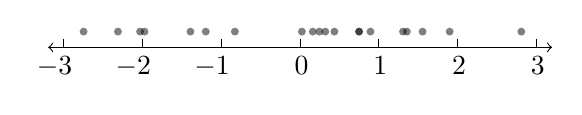
\begin{tikzpicture}
        \draw[<->] (-3.2, -0.2) -- (3.2, -0.2);
        \foreach \x in {-3, ..., 3} {
          \draw (\x, -0.2) -- (\x, -0.1);
          \draw (\x, -0.2) node[anchor=north east,xshift=0.23cm] {$\x$};
        }
        \foreach \x in {1.555, 1.899, 0.893, 0.160, 0.244, -0.829,
                        -1.199, -2.750, 0.022, -2.314, 2.809, 0.319,
                        -2.033, -1.976, 1.355, 0.749, 0.435, -1.393,
                        0.748, 1.306} {
          \fill[black,fill opacity=0.5] (\x,0) circle (0.05cm);
        }
      \end{tikzpicture}
      &
      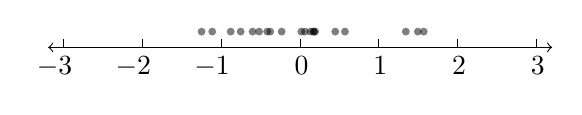
\begin{tikzpicture}
        \draw[<->] (-3.2, -0.2) -- (3.2, -0.2);
        \foreach \x in {-3, ..., 3} {
          \draw (\x, -0.2) -- (\x, -0.1);
          \draw (\x, -0.2) node[anchor=north east,xshift=0.23cm] {$\x$};
        }
        \foreach \x in {0.015, -0.418, 1.494, -0.882, 0.446, 0.061,
                        1.570, -0.755, 0.174, -0.604, -1.116, -0.380,
                        0.133, 0.569, -0.235, -0.521, 0.191, 0.169,
                        -1.252, 1.342} {
          \fill[black,fill opacity=0.5] (\x,0) circle (0.05cm);
        }
      \end{tikzpicture}
    \end{tabular}
  \end{center}
%   \begin{caption*}\end{caption*}
\end{figure}

In hierdie afdeling sal ons na die spreiding (dispersie) van ‘n datastel  kyk. Spreiding is ’n algemene term wat beskryf hoe die datawaardes uitgesprei is rondom die middel.
\par
\mindsetvid{Range and other measures of dispersion}{VMbsf}

\subsection{Variasiewydte}
\Definition{Variasiewydte}{Die variasiewydte van ’n datastel in die verskil tussen die maksiumum en die minimumwaardes in die stel.}

Die mees voor die handliggende  maatstaf van dispersie is die variasiewydte. Die variasiewydte dui aan hoe ver die grootste en die kleinste waardes in ’n datastel van mekaar verwyder is. Die variasiewydte is baie sensitief vir uitskieters.

\begin{wex}{Variasiewydte}
{Vind die variasiewydte van die volgende datastel:
    \begin{equation*}
      \{1;\ 4;\ 5;\ 8;\ 6;\ 7;\ 5;\ 6;\ 7;\ 4;\ 10;\ 9;\ 10\}
    \end{equation*}
    Wat sou gebeur as ons die eerste waarde in die datastel verwyder?
}{
  \westep{Vind die variasiewydte}
  Die kleinste waarde in die datastel is $1$ en die grootste waarde is $10$.\\
  Die variasiewydte is $10-1=9$.

  \westep{Verwyder die eerste datapunt}
  Ons doen dit nie gewoonlik nie, maar indien die eerste datapunt, 1, verwyder sou word uit die stel, sou die minimumwaarde verander van $1$ na $4$. Dit beteken dat die variasiewydte sou verander na $10- 4 = 6$. Dit verskil heelwat van die vorige variasiewyde; daarom sê ons dat die variasiewydte baie sensitief vir uitskieters is. In die datastel hierbo, was $1$ nie tipies van die hele stel datawaardes nie. Dit is ’n uitskieter en het ’n groot invloed op die variasiewydte. 
}
\end{wex}


\subsection{Persentiele}

\Definition{Persentiele}{Die $p^{de}$ persentiel is die waarde, $v$, wat die datastel in twee verdeel op so ’n manier dat $p$ persent van die waardes in die datastel minder is as $v$ en $100-p$ persent groter is as $v$. Persentiele kan lê in die variasiewydte $0 \leq  p \leq 100$.}

Om persentiele behoorlik te verstaan, moet ons tussen drie verskillende aspekte van ’n datapunt onderskei, naamlik: sy waarde, sy rangorde en sy persentiel:
\begin{itemize}
 \item Die waarde van ’n datapunt is dit wat ons meet of bepaal en aanteken gedurende ’n eksperiment of ondersoek.
\item Die rangorde van ’n datapunt is sy posisie in die gesorteerde datastel (dit wil sê eerste, tweede, derde ens.)  
\item Die persentiel waarby ’n bepaalde datapunt lê, sê vir ons watter persentasie van die waardes in die datastel minder is as hierdie betrokke punt.
\end{itemize}
\par
   Die tabel hieronder som die waardes, rangordes en persentiele van die datastel op:
  \begin{equation*}
    \{14,2;\ 13,9;\ 19,8;\ 10,3;\ 13,0;\ 11,1\}
  \end{equation*}

  \begin{center}
    \begin{tabular}{|c|c|c|} \hline

      \textbf{Waarde} & \textbf{Rangorde} & \textbf{Persentiele} \\\hline

      $10,3$  & $1$    & $0$ \\\hline
      $11,1$  & $2$    & $20$ \\\hline
      $13,0$  & $3$    & $40$ \\\hline
      $13,9$  & $4$    & $60$ \\\hline
      $14,2$  & $5$    & $80$ \\\hline
      $19,8$  & $6$    & $100$ \\\hline

    \end{tabular}
  \end{center}

 Let daarop dat die rangorde die volgorde van die datapunte beskryf, van die kleinste tot die grootste. Byvoorbeeld, $13,0$ is by die $40^{ste}$ persentiel aangesien daar $2$ waardes is wat minder is as $13,0$ en $3$ waardes wat groter is as $13,0$. 
  \begin{equation*}
    \frac{2}{2+3} = 0,4 = 40\%
  \end{equation*}
% \end{example}

In die algemeen kan ons sê dat die formule vir die vind van die $p^{de}$ persentiel in ’n geordende datastel met $n$ waardes, is: 
\begin{equation*}
  r = \frac{p}{100}\left(n-1\right)+1
\end{equation*}
Dit gee vir ons die rangorde, $r$, van die $p^{de}$ persentiel. Om die waarde van die $p^{de}$ persentiel te vind, tel ons vanaf die eerste waarde in die geordende datastel tot by die $r^{de}$ waarde.

Soms is die rangorde nie ’n heelgetal nie wat beteken die persentiel lê tussen twee waardes in die datastel. Die konvensie is om die waarde te neem halfpad tussen die twee waardes aangedui deur die rangorde.

 Die figuur hieronder toon die verwantskap tussen die rangorde en die persentiel grafies. Ons het reeds met drie persentiele te doen gekry: die mediaan ($50^{ste}$ persentiel), die minimum ($0^{de}$ persentiel) en die maksimum ($100^{ste}$).
\begin{center}
  \begin{tikzpicture}[xscale=0.1]
    \draw (0,0) -- (100,0);
    \foreach \p in {0, 25, ..., 100} {
      \draw (\p, -0.1) -- (\p, 0.1);
    }
    \draw (0, -0.1) node[anchor=north east,xshift=-0.35cm,yshift=-0.05cm] {$p$};
    \draw (0, -0.1) node[anchor=north] {$0$};
    \draw (50, -0.1) node[anchor=north] {$50$};
    \draw (100, -0.1) node[anchor=north] {$100$};
    \draw (0, -0.75) node[anchor=north] {minimum};
    \draw (50, -0.75) node[anchor=north] {mediaan};
    \draw (100, -0.75) node[anchor=north] {maksimum};
    \draw (0, +0.1) node[anchor=south east,xshift=-0.35cm,yshift=+0.05cm] {$r$};
    \draw (0, +0.1) node[anchor=south] {$1$};
    \draw (50, +0.1) node[anchor=south] {$\dfrac{n+1}{2}$};
    \draw (100, +0.1) node[anchor=south] {$n$};
  \end{tikzpicture}
\end{center}

%  Since $50\% = \frac{1}{2}$, the median is exactly the same as the $50^{\mathrm{th}}$
% percentile.  The minimum value is by definition the smallest and
% therefore the leftmost value in a sorted set. This makes the minimum
% equivalent to the $0^{\mathrm{th}}$ percentile. Similarly, the maximum is
% equivalent to the $100^{\mathrm{th}}$ percentile.

\begin{wex}{Gebruik die persentielformule}
{Pas die persentielformule toe en bepaal die minimum, maksimum en mediaanwaardes van die volgende datastel. 
    \begin{equation*}
      \{14;\ 17;\ 45;\ 20;\ 19;\ 36;\ 7;\ 30;\ 8\}
    \end{equation*}
}{
    \westep{Sorteer die waardes in die datastel}

  Heel eerste moet ons die datastel sorteer van die kleinste tot die grootste:
    \begin{equation*}
      \{7;\ 8;\ 14;\ 17;\ 19;\ 20;\ 30;\ 36;\ 45\}
    \end{equation*}

    \westep{Vind die minimum}

    Die minimum is die eerste waarde in die geordende datastel. Ons gaan nou bevestig dat die persentielformule dieselfde resultaat gee. Die minimum is ekwivalent aan die $0^{de}$ persentiel. Volgens die formule is die rangorde, $r$, van die $0^{de}$ persentiel in ’n datastel met $9$ datawaardes:
    \begin{align*}
      r &= \frac{p}{100}\left(n-1\right)+1 \\
        &= \frac{0}{100}\left(9-1\right)+1 \\
        &= 1
    \end{align*}
    Dit bevestig die minimumwaarde is die eerste waarde in die datastel, naamlik $7$.

    \westep{Vind die maksimum}

    Die maksimumwaarde is die laaste waarde in die geordende datastel en dit is ekwivalent aan die $100^{ste}$
    persentiel. Met gebruik van die formule met $p=100$ en $n=9$,
     vind ons die rangorde van die maksimumwaarde as
    \begin{align*}
      r &= \frac{p}{100}\left(n-1\right)+1 \\
        &= \frac{100}{100}\left(9-1\right)+1 \\
        &= 9
    \end{align*}
    Dit bevestig die maksimumwaarde is die laaste ($9^{de}$) waarde in die lys, naamlik $45$.

    \westep{Vind die mediaan}

    Die mediaan is ekwivalent aan die $50^{ste}$ persentiel. Met gebruik van die formule met $p=50$ en $n=9$, vind ons die rangorde van die mediaanwaarde as
    \begin{align*}
      r &= \frac{50}{100}\left(n-1\right)+1 \\
        &= \frac{50}{100}\left(9-1\right)+1 \\
        &= \frac{1}{2}(8)+1 \\
        &= 5
    \end{align*}
    Dit bevestig die mediaanwaarde is die middelste $50^{ste}$ waarde in die gesorteerde datastel, naamlik $19$. 
}
\end{wex}

\Definition{Kwartiele}{Die kwartiele is die drie datawaardes wat die gesorteerde datastel in vier groepe verdeel, waar elk van die groepe ’n gelyke aantal datawaardes bevat. Die mediaan  ($50^{ste}$
  persentiel) is die tweede kwartiel. Die $25^{ste}$ persentiel word ook die onderste (laer) kwartiel genoem ($Q1$), en die $75^{ste}$ persentiel, die boonste (ho\"er) kwartiel ($Q3$).}

\begin{wex}{Kwartiele}
{Bepaal die kwartiele van die volgende datastel:
    \begin{equation*}
      \{7;\ 45;\ 11;\ 3;\ 9;\ 35;\ 31;\ 7;\ 16;\ 40;\ 12;\ 6\}
    \end{equation*}
}{
    \westep{Sorteer die datastel}
    \begin{equation*}
      \{3;\ 6;\ 7;\ 7;\ 9;\ 11;\ 12;\ 16;\ 31;\ 35;\ 40;\ 45\}
    \end{equation*}

    \westep{Vind die rangordes van die kwartiele}

    Met gebruik van die persentielformule, vind ons die rangordes van die $25^{ste}$,
    $50^{ste}$ en $75^{ste}$ persentiele as:
    \begin{align*}
      r_{25} &= \frac{25}{100}\left(12-1\right)+1 \\
            &= 3,75 \\
      r_{50} &= \frac{50}{100}\left(12-1\right)+1 \\
            &= 6,5 \\
      r_{75} &= \frac{75}{100}\left(12-1\right)+1 \\
            &= 9,25
    \end{align*}

    \westep{Vind die waardes van die kwartiele}

    Let daarop dat elk van van hierdie rangordes ’n breuk is, wat beteken dat die waarde vir elke persentiel iewers tussen twee waardes op die datastel lê. \par

    Vir die $25^{ste}$ persentiel is die rangorde $3,75$, tussen die $3^{de}$ en $4^{de}$ waardes. Aangesien beide van hierdie waardes gelyk is aan 
    $7$, is die $25^{ste}$ persentiel $7$.\par

    Die rangorde vir die $50^{ste}$ persentiel (die mediaan) is $6,5$, halfpad tussen die  $6^{de}$ en $7^{de}$ waardes. Die $6^{de}$ waarde is
    $11$ en die $7^{de}$ waarde is $12$, wat beteken die mediaan is
    \(\frac{11+12}{2} = 11,5\).\par

    Die rangrode vir die $75^{ste}$ persentiel is die rangorde $9,25$, halfpad tussen die
    $9^{de}$ en $10^{de}$ waardes. Dus die $75^{ste}$ persentiel is
    \(\frac{31+35}{2} = 33\).\par
  }
\end{wex}
%english
\subsubsection*{Desiele}
Die desiele is die nege datawaardes wat 'n geordende stel data in tien groepe verdeel, waar elke groep bevat 'n gelyke aantal datawaardes bevat.

\par
Byvoorbeeld, beskou die geordende stel data:
\begin{center}
$28; 33; 35; 45; 57; 59; 61; 68; 69; 72; 75; 78; 80; 83; 86; 91;$ \\ 
$92; 95; 101; 105; 111; 117; 118; 125; 127; 131; 137; 139; 141$\\
\end{center}
Die nege desiele is: $35; 59; 69; 78; 86; 95; 111; 125; 137$


\subsection{Persentiele vir gegroepeerde data}

In gegroepeerde data sal die persentiele iewers in ‘n interval lê, eerder as by ’n spesifieke waarde. Om die interval te vind waarbinne die persentiel lê, gebruik ons weereens die persentielformule om die rangorde van die persentiel te vind en dan kry ons die interval waarbinne die rangorde l\^e.

\begin{wex}{Persentiele in gegroepeerde data}
{Die wiskundepunte van $100$ graad $10$ leerders by ’n skool is ingesamel en die data voorgestel in die volgende tabel:\\
    \begin{center}
      \begin{tabular}{|c|c|}  \hline
       
       \textbf{Persentasiepunt} & \textbf{Aantal leerders} \\  \hline

         $0$  $ \leq x < $   $20$ &  $2$ \\ \hline
        $20$  $ \leq x < $   $30$ &  $5$ \\\hline
        $30$  $ \leq x < $   $40$ & $18$ \\\hline
        $40$  $ \leq x < $   $50$ & $22$ \\\hline
        $50$  $ \leq x < $   $60$ & $18$ \\\hline
        $60$  $ \leq x < $   $70$ & $13$ \\\hline
        $70$  $ \leq x < $   $80$ & $12$ \\\hline
        $80$  $ \leq x < $  $100$ & $10$ \\\hline
   
      \end{tabular}
    \end{center}
\vspace {8pt}\\
\begin{minipage}{\textwidth}
    \begin{enumerate}[noitemsep, label=\textbf{\arabic*}.]
    \item Bereken die gemiddelde van hierdie gegroepeerde datastel.
    \item In watter intervalle is die kwartiele van hierdie datastel?
    \item In watter interval is die $30^{ste}$ persentiel van die datastel?
    \end{enumerate}
\end{minipage}
}{
  \westep{Bereken die gemiddelde}

  Aangesien ons die gegroepeerde data het en nie die oorspronklike ongegroepeerde data nie, is die beste wat ons kan doen om die benaderde waarde van die gemiddelde te bereken asof al die leerders in elke interval in die middel van die interval l\^e.

  \begin{align*}
 \mbox{Gemid. } &=  \frac{
         2\:.\:10
      +  5\:.\:25
      + 18\:.\:35
      + 22\:.\:45
      + 18\:.\:55
      + 13\:.\:65
      + 12\:.\:75
      + 10\:.\:90
    }{100}\\
    &= 54\%
  \end{align*}

  \westep{ Vind die kwartiele}

  Die data is reeds gegroepeer, dus is dit ook gesorteer. Gebruik die persentielformule en die feit dat daar
  $100$ leerders is om die rangorde van die $25^{ste}$, $50^{ste}$ en
  $75^{ste}$ persentiele te vind:
  \begin{align*}
    r_{25} &= \frac{25}{100}\left(100-1\right)+1 \\
          &= 24,75 \\
    r_{50} &= \frac{50}{100}\left(100-1\right)+1 \\
          &= 50,5 \\
    r_{75} &= \frac{75}{100}\left(100-1\right)+1 \\
          &= 75,25
  \end{align*}

  Nou moet ons die intervalle kry waarbinne hierdie rangordes val.

\hspace*{-40pt}
\begin{minipage}{0.85\textwidth}
\vspace*{10pt}


  \begin{itemize}
  \item Vir die onderste kwartiel vind ons daar is $2 + 5 = 7$ leerders in die onderste twee intervalle gekombineerd en $2 + 5 + 18 = 25$
    in die eerste drie intervalle. Dit beteken die onderste kwartiel, met
    $7 < r_{25} < 25$,
    lê iewers in die derde interval: $30 \leq x < 40$.
  \item Vir die tweede kwartiel (die mediaan) het ons
    $2 + 5 + 18 + 22 = 47$ leerders in die eerste vier intervalle gekombineerd en $65$ leerders in die eerste 5 intervalle. Dit beteken die mediaan, met $47 < r_{50} < 65$,
    l\^e iewers in die vyfde interval: $50 \leq x < 60$.
  \item Vir die boonstel kwartiel, het ons $65$ leerders in die eerste vyf intervalle gekombineerd en  $65 + 13 = 78$ 
    leerders in die eerste ses intervalle. Dit beteken die boonste kwartiel, met rangorde,
    $65 < r_{75} < 78$,
    l\^e iewers in die sesde interval: $60 \leq x < 70$.
  \end{itemize}
\end{minipage}
  \westep{ Vind die $30^{ste}$ persentiel}

  Gebruik dieselfde metode as vir die kwartiele om die rangorde van die $30^{ste}$ persentiel te vind.
  \begin{align*}
    r &= \frac{30}{100}\left(100-1\right)+1 \\
      &= 30,7
  \end{align*}
  Nou vind ons die interval waarbinne die rangorde l\^e. Aangesien daar $25$ leerders is in die eerste $3$ intervalle altesaam en $47$
  in die eerste vier intervalle , l\^e die $30^{ste}$ persentiel in die vierde interval $40 \leq x < 50$.
}
\end{wex}

\subsection{Variasiewydtes}
Ons definieer die variasiewydtes in terme van die persentiele. Ons het reeds die variasiewydte van die hele datastel gedefineer as die verskil tussen die 
$100^{ste}$ persentiel en die $0^{de}$ persentiel (dit wil sê tussen die maksimum- en die minimumwaardes in die datastel).

\Definition{Interkwartielwydte}{Die interkwartielwydte is ’n maatstaf van spreiding wat bereken word deur die onderste (eerste) kwartiel ($Q1$) van die boonste (hoër) kwartiel ($Q3$) af te trek. Dit gee die wydte van die middelste helfte van die datastel.
}

\Definition{Semi-interkwartielwydte}{Die semi-interkwartielwydte is die helfte van die interkwartielwydte.}

\begin{exercises}{}{
  \begin{enumerate}[noitemsep, label=\textbf{\arabic*}.]

  \item Vind die variasiewydte van die datastel:
    \begin{equation*}
      \{1;\ 2;\ 3;\ 4;\ 4;\ 4;\ 5;\ 6;\ 7;\ 8;\ 8;\ 9;\ 10;\ 10\}
    \end{equation*}

  \item Wat is die kwartiele van hierdie datastel?
    \begin{equation*}
      \{3;\ 5;\ 1;\ 8;\ 9;\ 12;\ 25;\ 28;\ 24;\ 30;\ 41;\ 50\}
    \end{equation*}

  \item ’n Klas van $12$ studente skryf ’n toets en die resultaat is as volg:
    \begin{equation*}
      20;\ 39;\ 40;\ 43;\ 43;\ 46;\ 53;\ 58;\ 63;\ 70;\ 75;\ 91
    \end{equation*}
    Vind die variasiewydte, kwartiele en die interkwartielwydte.

  \item Drie stelle data word gegee:
    \begin{itemize}  
    \item \textbf{Datastel 1:} $\{9;\ 12;\ 12;\ 14;\ 16;\ 22;\ 24\}$
    \item \textbf{Datastel 2:} $\{7;\ 7;\ 8;\ 11;\ 13;\ 15;\ 16;\ 16\}$
    \item \textbf{Datastel 3:} $\{11;\ 15;\ 16;\ 17;\ 19;\ 19;\ 22;\ 24;\ 27\}$
    \end{itemize}
    Vir elke datastel vind:
    \begin{enumerate}[noitemsep, label=\textbf{(\alph*)} ]
    \item die variasiewydte
    \item die onderste kwartiel
    \item die interkwartielwydte
    \item die semi-interkwartielwydte
    \item die mediaan
    \item die boonste kwartiel
    \end{enumerate}
  \end{enumerate}
% Automatically inserted shortcodes - number to insert 4
\par \practiceinfo
\par \begin{tabular}[h]{cccccc}
% Question 1
(1.)	02r0	&
% Question 2
(2.)	02r1	&
% Question 3
(3.)	02r2	&
% Question 4
(4.)	02r3	&
\end{tabular}
% Automatically inserted shortcodes - number inserted 4
% \practiceinfo
% \par 
% \par \begin{tabular}[h]{cccccc}
% (1.) 00k0&  (2.) 00k1&  (3.) 00k2&  (4.) 00k3& \end{tabular}
}
\end{exercises}

\section{Vyf-getal opsomming}
’n Algemene manier om ’n totale datastel op te som is met die vyf-getal opsomming en die ‘mond-en-snor’ grafiek (in Engels ‘box-and-whisker plot’). Hierdie twee voorstellings verteenwoordig presies dieselfde inligting, numeries in die geval van die vyf-getal opsomming en grafies in die geval van die mond-en-snor grafiek.

\par
Die vyf-getal opsomming bestaan uit die minimumwaarde, die maksimumwaarde en die drie kwartiele. Ons kan ook sê dit bestaan uit die $0^{de}$,
$25^{ste}$, $50^{ste}$, $75^{ste}$, $100^{ste}$ persentiele.

Die mond-en-snor grafiek toon die vyf persentiele soos in die figuur hieronder. Die mond-reghoek wys die interkwartiel wydte (die afstand tussen die  $Q1$ en $Q3$). ’n Lyn binne-in hierdie reghoek toon die mediaan (die tweede kwartiel). Die lyne wat uitsteek aan die kante van die mond-reghoek (dit is die snor-gedeeltes) wys waar die maksimum- en minimumwaardes lê. 
\par
\mindsetvid{Box and whisker plot}{VMbur}
\clearpage
\begin{figure}[t]
  \begin{center}
    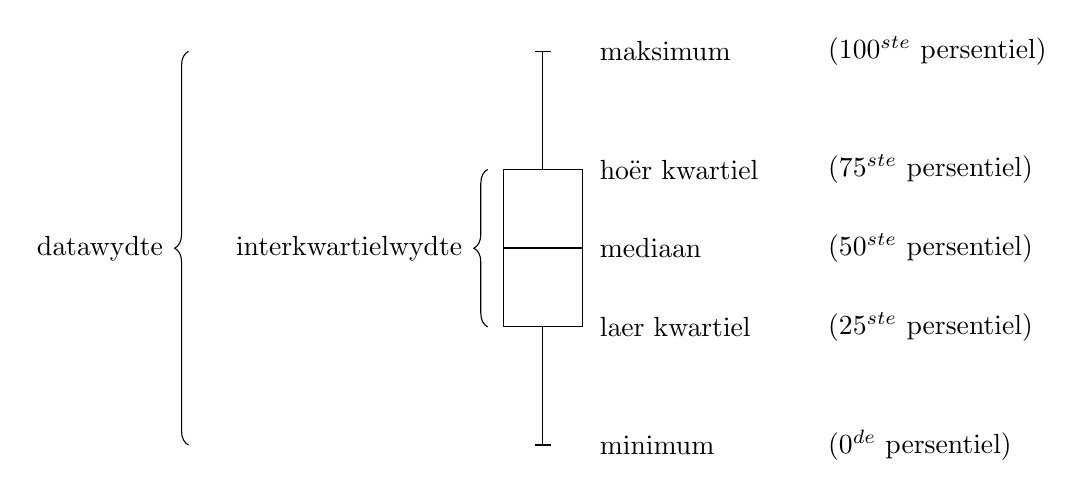
\begin{tikzpicture}
      \draw[thick] (-0.5, 0) -- (0.5, 0);
      \draw (-0.5, -1) rectangle (0.5, 1);
      \draw (0, -1) -- (0, -2.5);
      \draw (-0.1, -2.5) -- (0.1, -2.5);
      \draw (0, 1) -- (0, 2.5);
      \draw (-0.1, 2.5) -- (0.1, 2.5);
      \draw (0.6, 2.5) node[anchor=west] {maksimum};
      \draw (0.6, 1) node[anchor=west] {ho\"er kwartiel};
      \draw (0.6, 0) node[anchor=west] {mediaan};
      \draw (0.6, -1) node[anchor=west] {laer kwartiel};
      \draw (0.6, -2.5) node[anchor=west] {minimum};
      \draw (3.5, 2.5) node[anchor=west] {($100^{ste}$ persentiel)};
      \draw (3.5, 1) node[anchor=west] {($75^{ste}$ persentiel)};
      \draw (3.5, 0) node[anchor=west] {($50^{ste}$ persentiel)};
      \draw (3.5, -1) node[anchor=west] {($25^{ste}$ persentiel)};
      \draw (3.5, -2.5) node[anchor=west] {($0^{de}$ persentiel)};
      \draw[decoration={brace,amplitude=0.5em},decorate] (-0.7,-1) -- (-0.7,1);
      \draw (-0.7,0) node[anchor=east,xshift=-0.2cm] {interkwartielwydte};
      \draw[decoration={brace,amplitude=0.5em},decorate] (-4.5,-2.5) -- (-4.5,2.5);
      \draw (-4.5,0) node[anchor=east,xshift=-0.2cm] {datawydte};
    \end{tikzpicture}
  \end{center}
%   \begin{caption*}The box-and-whisker plot along with labels showing how
%     the different percentiles and ranges are represented in the plot.\end{caption*}
\end{figure}
\vspace{1cm}

\begin{wex}{Vyf-getal opsomming}
{Trek ’n mond-en-snor grafiek van die volgende datastel:
    \begin{equation*}
      \{1,25;\ 1,5;\ 2,5;\ 2,5;\ 3,1;\ 3,2;\ 4,1;\ 4,25;\ 4,75;\ 4,8;\ 4,95;\ 5,1\}
    \end{equation*}
}{
  \westep{Bepaal die minimum en die maksimum}

  Aangesien die datastel reeds gesorteer is, kan ons die minimum aflees as die eerste waarde ($1,25$) en die maksimum as die laaste waarde ($5,1$).

  \westep{Bepaal die kwartiele}

  Daar is $12$ waardes in die datastel. Met die persentielformule, kan ons bepaal die mediaan lê tussen die $6^{de}$ en die $7^{de}$
  waardes, dus
  \begin{equation*}
    \frac{3,2 + 4,1}{2} = 3,65
  \end{equation*}

  Die eerste kwartiel lê tussen die $3^{de}$ en $4^{de}$ waardes en dit gee
  
  \begin{equation*}
    \frac{2,5 + 2,5}{2} = 2,5
  \end{equation*}

  Die derde kwartiel lê tussen die $9^{de}$ and $10^{de}$ waardes en dit gee
  
  \begin{equation*}
    \frac{4,75 + 4,8}{2} = 4,775
  \end{equation*}

 Dit gee die data vir die vyf-getal opsomming en die datastel stel ons in staat om die mond-en-snor grafiek te trek.

  \begin{center}
    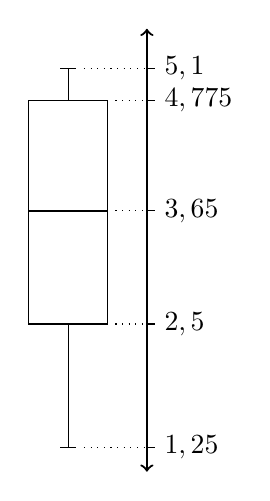
\begin{tikzpicture}[yscale=1.25]
      \def\median{3.65}
      \def\firstquartile{2.5}
      \def\thirdquartile{4.775}
      \def\minimum{1.25}
      \def\maximum{5.1}

      \draw (-0.5, \firstquartile) rectangle (0.5, \thirdquartile);
      \draw[thick] (-0.5, \median) -- (0.5, \median);
      \draw (0,    \firstquartile) -- (0,   \minimum);
      \draw (-0.1, \minimum) -- (0.1,       \minimum);
      \draw (0,    \thirdquartile) -- (0,   \maximum);
      \draw (-0.1, \maximum) -- (0.1,       \maximum);

      \draw[thick,<->] (1,1) -- (1,5.5);

      \foreach \y in {\minimum, \firstquartile, \median, \thirdquartile, \maximum} {
        \draw (1, \y) -- (1.1, \y);
      }
      \foreach \y/\txt in {\minimum/{1,25}, \firstquartile/{2,5}, \median/{3,65}, \thirdquartile/{4,775}, \maximum/{5,1}} {
        \draw (1.1, \y) node[anchor=west] {$\txt$};
      }
      \draw[dotted] (0.2, \maximum) -- (1, \maximum);
      \draw[dotted] (0.6, \thirdquartile) -- (1, \thirdquartile);
      \draw[dotted] (0.6, \median)  -- (1, \median);
      \draw[dotted] (0.6, \firstquartile) -- (1, \firstquartile);
      \draw[dotted] (0.2, \minimum) -- (1, \minimum);
    \end{tikzpicture}
  \end{center}
}
\end{wex}

\begin{exercises}{}{
    \begin{enumerate} [itemsep=6pt, label=\textbf{\arabic*}.]

    \item Lisa werk in ’n rekenaarwinkel. Sy verkoop die volgende aantal rekenaars in ’n maand:
      \begin{equation*}
        \{27;\ 39;\ 3;\ 15;\ 43;\ 27;\ 19;\ 54;\ 65;\ 23;\ 45;\ 16\}
      \end{equation*}
     Gee die vyf-getal opsomming en die mond-en-snor grafiek van Lisa se verkope.

    \item Zithulele werk in telefoonverkope. Hy hou boek van die aantal verkope wat hy elke maand doen en die data word hier gegee:.
      \begin{equation*}
        \{49;\ 12;\ 22;\ 35;\ 2;\ 45;\ 60;\ 48;\ 19;\ 1;\ 43;\ 12\}
      \end{equation*}
    Gee die vyf-getal opsomming en die mond-en-snor grafiek van Zithulele se verkope.

    \item Hannah het vir nege maande gewerk as ’n bloemiste. Sy verkoop die volgende aantal bruidsruikers:
      \begin{equation*}
        \{16;\ 14;\ 8;\ 12;\ 6;\ 5;\ 3;\ 5;\ 7\}
      \end{equation*}
      Gee die vyf-getal opsomming van Hannah se verkope.
    \item Gebruik die diagram hieronder om die vyf-getal opsomming te bereken:
      \begin{enumerate}[noitemsep, label=\textbf{(\alph*)} ]
      \item \raisebox{-2cm}{
          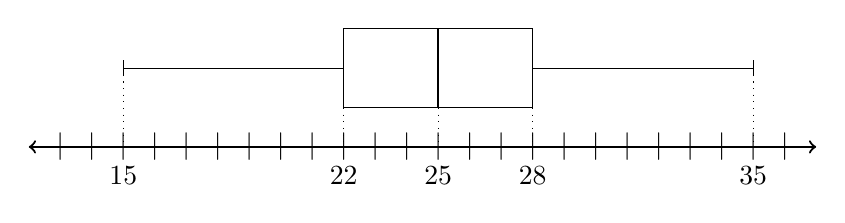
\begin{tikzpicture}[xscale=0.4]
            \def\median{25}
            \def\firstquartile{22}
            \def\thirdquartile{28}
            \def\minimum{15}
            \def\maximum{35}

            \draw (\firstquartile, -0.5 ) rectangle ( \thirdquartile,0.5);
            \draw[thick] ( \median,-0.5) -- ( \median,0.5);
            \draw (    \firstquartile, 0) -- (\minimum,0   );
            \draw ( \minimum, -0.1) -- (       \minimum, 0.1);
            \draw (  \thirdquartile, 0) -- (   \maximum, 0);
            \draw ( \maximum, -0.1) -- (      \maximum, 0.1 );

            \draw[thick,<->] (12,-1) -- (37,-1);

            \foreach \x in {\minimum, \firstquartile, \median, \thirdquartile, \maximum} {
              \draw (\x,-1.6) -- (\x, -1.6) node[anchor=south] {$\x$};
            }

            \foreach \x in {13,14,...,36} {
              \draw (\x,-1.3) -- (\x, -1.3) node[anchor=south] {$|$};
            }
            \draw[dotted] ( \maximum, 0) -- ( \maximum, -1);
            \draw[dotted] ( \thirdquartile, 0) -- ( \thirdquartile, -1);
            \draw[dotted] (\median, 0)  -- ( \median, -1);
            \draw[dotted] (\firstquartile, 0) -- ( \firstquartile, -1);
            \draw[dotted] ( \minimum, 0) -- ( \minimum, -1);
          \end{tikzpicture}
        }
      \item \raisebox{-2cm}{
          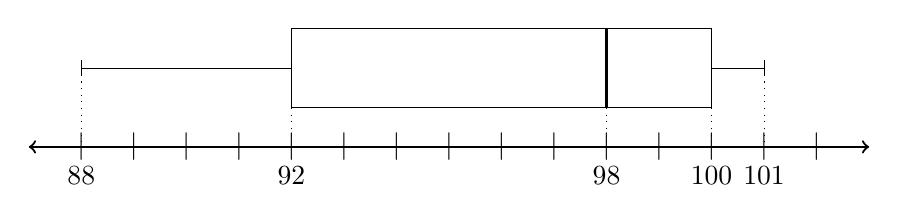
\begin{tikzpicture}[xscale=0.667]
            \def\median{98}
            \def\firstquartile{92}
            \def\thirdquartile{100}
            \def\minimum{88}
            \def\maximum{101}

            \draw (\firstquartile, -0.5 ) rectangle ( \thirdquartile,0.5);
            \draw[thick] ( \median,-0.5) -- ( \median,0.5);
            \draw (    \firstquartile, 0) -- (\minimum,0   );
            \draw ( \minimum, -0.1) -- (       \minimum, 0.1);
            \draw (  \thirdquartile, 0) -- (   \maximum, 0);
            \draw ( \maximum, -0.1) -- (      \maximum, 0.1 );

            \draw[thick,<->] (87,-1) -- (103,-1);

            \foreach \x in {\minimum, \firstquartile, \median, \thirdquartile, \maximum} {
              \draw (\x,-1.6) -- (\x, -1.6) node[anchor=south] {$\x$};
            }

            \foreach \x in {88,89,...,102} {
              \draw (\x,-1.3) -- (\x, -1.3) node[anchor=south] {$|$};
            }
            \draw[dotted] ( \maximum, 0) -- ( \maximum, -1);
            \draw[dotted] ( \thirdquartile, 0) -- ( \thirdquartile, -1);
            \draw[dotted] (\median, 0)  -- ( \median, -1);
            \draw[dotted] (\firstquartile, 0) -- ( \firstquartile, -1);
            \draw[dotted] ( \minimum, 0) -- ( \minimum, -1);
          \end{tikzpicture}
        }
      \end{enumerate}
    \end{enumerate}
% Automatically inserted shortcodes - number to insert 4
\par \practiceinfo
\par \begin{tabular}[h]{cccccc}
% Question 1
(1.)	02r4	&
% Question 2
(2.)	02r5	&
% Question 3
(3.)	02r6	&
% Question 4
(4.)	02r7	&
\end{tabular}
% Automatically inserted shortcodes - number inserted 4
% \practiceinfo
% \par 
% \par \begin{tabular}[h]{cccccc}
% (1.) 00k4&  (2.) 00k5&  (3.) 00k6&  (4.) 00k7\end{tabular}
}
\end{exercises}


\summary{VMdvy}

\begin{itemize}[itemsep=6pt]
\item Data verwys na stukke inligting wat waargeneem en opgeteken is in ’n eksperiment of
opname. 

\item Kwantitatiewe data kan as getalle geskryf word. Kwantitatiewe data kan diskreet of kontinu wees.

\item Kwalitatiewe data is data wat nie as getalle geskryf kan word nie. Kategoriale data en anekdotiese data is twee algemene tipes kwalitatiewe data.

\item Die gemiddelde word gedefinieer as die som van ’n stel datawaardes, gedeel deur
die aantal waardes in die som. 
  \begin{align*}
    \overline{x} &= \frac{1}{n}\sum_{i=1}^n x_i \\
                 &= \frac{x_1 + x_2 + \cdots + x_n}{n}
  \end{align*}

\item Die mediaan van ’n datastel is die waarde van die sentrale of middelste datapunt
wanneer die datastel georden word van die kleinste tot die grootste waarde. As daar ’n ewe aantal datapunte is sal die mediaan halfpad tussen twee waardes in die datastel wees.
 

\item Die modus van ’n datastel is die waarde wat die meeste voorkom in die stel. 

\item ’n Uitskieter is ’n waarde in die datastel wat nie tipies is van die res van die stel
nie. Dit is gewoonlik ’n waarde wat baie groter of baie kleiner is as al die ander
waardes in die stel.

\item Spreiding is ’n algemene term wat beskryf hoe die datawaardes uitgesprei is rondom die middel.

\item Die variasiewydte van ’n datastel in die verskil tussen die maksiumum- en minimumwaardes in die stel. 

\item Die $p^{de}$ persentiel is die waarde, $v$ , wat die datastel in twee verdeel op so ’n manier dat $p$ persent van die waardes in die datastel minder is as $v$ en $100 − p$ persent groter is as $v$.


Die formule vir die vind van die $p^{de}$ persentiel in ’n geordende datastel met $n$ waardes is:
\begin{equation*}
  r = \frac{p}{100}\left(n-1\right)+1
\end{equation*}

\item Die kwartiele is die drie datawaardes wat die gesorteerde datastel in vier groepe verdeel, waar elk van die groepe ’n gelyke aantal datawaardes bevat. Die onderste kwartiel is ($Q1$), die mediaan ($Q2$) en die boonste kwartiel ($Q3$).

\item Die interkwartielwydte is ’n maatstaf van spreiding wat bereken word deur die onderste kwartiel ($Q1$) van die boonste kwartiel ($Q3$) af te trek. Dit gee die wydte van die middelste helfte van die datastel.

\item Die semi-interkwartielwydte is die helfte van die interkwartielwydte. 

\item Die vyf-getal opsomming bestaan uit die minimumwaarde, die maksimumwaarde en die drie kwartiele ($Q1$, $Q2$ en $Q3$). 

\item Die mond-en-snor grafiek toon vyf persentiele.
\end{itemize}

\begin{eocexercises}{}
  \begin{enumerate}[itemsep=6pt, label=\textbf{\arabic*}.]

  \item 
  Die hoogste $7$ bome in die park het hoogtes (in meters): 
\begin{center} 
 $41$; $60$; $47$; $42$; $44$; $42$; $47$  
\end{center}
Vind die mediaan van hulle hoogtes.

  \item Die studente in Ndeme se klas het die volgende ouderdomme:
    \begin{center} 
$5$; $6$; $7$; $5$; $4$; $6$; $6$; $6$; $7$; $4$ 
    \end{center}
Vind die modale ouderdom.

  \item ’n Ingenieursfirma het twee tipes enjins vir motorfietse ontwerp. Die twee motorfietse word getoets vir die tyd (in sekondes) wat dit hulle neem om te versnel van $0$
    km/h tot $60$ km/h.

    \begin{center}
\hspace*{-50pt}
      \begin{tabular}{|@{\hspace{0.1cm}}c@{\hspace{0.1cm}}|@{\hspace{0.1cm}}c@{\hspace{0.1cm}}|@{\hspace{0.1cm}}c@{\hspace{0.1cm}}|@{\hspace{0.1cm}}c@{\hspace{0.1cm}}|@{\hspace{0.1cm}}c@{\hspace{0.1cm}}|@{\hspace{0.1cm}}c@{\hspace{0.1cm}}|@{\hspace{0.1cm}}c@{\hspace{0.1cm}}|@{\hspace{0.1cm}}c@{\hspace{0.1cm}}|@{\hspace{0.1cm}}c@{\hspace{0.1cm}}|@{\hspace{0.1cm}}c@{\hspace{0.1cm}}|@{\hspace{0.1cm}}c@{\hspace{0.1cm}}|} \hline
     
        & \textbf{Toets 1} & \textbf{Toets 2} & \textbf{Toets 3} & \textbf{Toets 4} & \textbf{Toets 5} & \textbf{Toets 6} & \textbf{Toets 7} &\textbf{Toets 8} & \textbf{Toets 9} & \textbf{Toets 10} \\\hline
        \textbf{Fiets 1} & $1,55$ & $1,00$ & $0,92$ & $0,80$ & $1,49$ & $0,71$ & $1,06$ & $0,68$ & $0,87$ & $1,09$ \\\hline
        \textbf{Fiets 2} & $0,9$ & $1,0$ & $1,1$ & $1,0$ & $1,0$ & $0,9$ & $0,9$ & $1,0$ & $0,9$ & $1,1$ \\\hline

      \end{tabular}
    \end{center}
\vspace {8pt}\\
\begin{enumerate}[noitemsep, label=\textbf{(\alph*)} ]
    \item Watter maatstaf van sentrale neiging behoort gebruik te word vir hierdie data?
    \item Bereken die maatstaf van sentrale neiging wat jy gekies het in (a), vir elke motorfiets.
    \item Watter motorfiets sou jy kies, gebaseer op hierdie inligting? Neem kennis van die akkuraatheid van die getalle in elke stel toetse. 
      
    \end{enumerate}

  \item In ’n verkeersopname, word ’n willekeurige steekproef van $50$ motoriste gevra oor die afstand wat hulle elke dag werk toe ry. Die informasie word getoon in die tabel hieronder: \\
    \begin{center}
      \begin{tabular}{|c|c|} \hline
     
        \textbf{Afstand (km)} & \textbf{Telling} \\ \hline

        $0 < d \leq 5$ & $4$ \\ \hline
        $5 < d \leq 10$ & $5$ \\\hline
        $10 < d \leq 15$ & $9$ \\\hline
        $15 < d \leq 20$ & $10$ \\\hline
        $20 < d \leq 25$ & $7$ \\\hline
        $25 < d \leq 30$ & $8$ \\\hline
        $30 < d \leq 35$ & $3$ \\\hline
        $35 < d \leq 40$ & $2$ \\\hline
        $40 < d \leq 45$ & $2$ \\\hline

      \end{tabular}
    \end{center}
\vspace {8pt}\\
     \begin{enumerate}[noitemsep, label=\textbf{(\alph*)} ]
    \item Vind die benaderde gemiddelde van die data.
    \item Watter persentasie van die steekproef ry 
      \begin{enumerate}[noitemsep, label=\textbf{\roman*}. ]
      \item minder as $15$ km?
      \item meer as $30$ km?
      \item tussen $16$ km en $30$ km daagliks?
      \end{enumerate}
\item Teken 'n histogram om die data voor te stel.
    \end{enumerate}

  \item ’n Maatskappy wil die opleidingsprogram in sy fabriek evalueer. Hulle gee dieselfde taakopdrag aan opgeleide en onopgeleide werknemers en meet die tyd in sekondes wat  dit die werkers neem om die taak te voltooi. 
\\
    \begin{center}
      \begin{tabular}{|l|c|c|c|c|c|} \hline

        \textbf{Opgeleide} & $121$ & $137$ & $131$ & $135$ & $130$ \\ \hline
                           & $128$ & $130$ & $126$ & $132$ & $127$ \\\hline
                           & $129$ & $120$ & $118$ & $125$ & $134$ \\\hline

        \textbf{Onopgeleide} & $135$ & $142$ & $126$ & $148$ & $145$ \\\hline
                             & $156$ & $152$ & $153$ & $149$ & $145$ \\\hline
                             & $144$ & $134$ & $139$ & $140$ & $142$ \\\hline

      \end{tabular}
    \end{center}
\vspace {8pt}\\
    \begin{enumerate}[noitemsep, label=\textbf{(\alph*)} ]
    \item Vind die mediane en kwartiele vir beide stelle data.
    \item Vind die interkwartielwydtes vir beide stelle data.
    \item Lewer kommentaar op die resultate.
\item Vir elke datastel teken 'n mond-en-snor diagram wat die vyf-getal-opsomming illustreer.
    \end{enumerate}

  \item ’n Klein firma het $9$ mense in diens. Die jaarlikse salarisse van die werknemers is:\\
    \begin{center}
      \begin{tabular}{|r|r|r|} \hline
        R~$600~000$ & R~$250~000$ & R~$200~000$ \\\hline
        R~$120~000$ & R~$100~000$ & R~$100~000$ \\\hline
        R~$100~000$ &  R~$90~000$ &  R~$80~000$ \\\hline
      \end{tabular}
    \end{center}
\vspace {8pt}\\
    \begin{enumerate}[noitemsep, label=\textbf{(\alph*)} ]
    \item Vind die gemiddelde van hierdie salarisse
    \item Vind die modus
    \item Vind die mediaan
    \item Watter een van die drie getalle sou jy gebruik om te onderhandel oor salarisverhogings as jy ’n vakbondbeampte is? Waarom?
    \end{enumerate}

  \end{enumerate}
% Automatically inserted shortcodes - number to insert 6
\par \practiceinfo
\par \begin{tabular}[h]{cccccc}
% Question 1
(1.)	02r8	&
% Question 2
(2.)	02r9	&
% Question 3
(3.)	02ra	&
% Question 4
(4.)	02rb	&
% Question 5
(5.)	02rc	&
% Question 6
(6.)	02rd	\\ % End row of shortcodes
\end{tabular}
% Automatically inserted shortcodes - number inserted 6
% \practiceinfo
% \par 
% \par \begin{tabular}[h]{cccccc}
% (1.) 00k8&  (2.) 00k9&  (3.) 00ka&  (4.) 00kb&  (5.) 00kc&  (6.) 00kd\end{tabular}
\end{eocexercises}
